\documentclass[a4paper,11pt]{article}
\usepackage[english, french]{babel}
\usepackage[utf8]{inputenc}

\usepackage{graphicx}
\usepackage{fancyhdr}
\usepackage{lastpage}

\usepackage{hyperref}
\usepackage{float}

\usepackage{array}

\usepackage[top=20mm, bottom=20mm, left=25mm, right=25mm]{geometry}


\title{Guide de style}

\begin{document}
\maketitle
\section{À propos de ce document}
Ce document présente les différentes conventions qui seront utilisées pour les
différents livrables du projet. Il servira à assurer l'uniformité du rendu des
documents, et devra être respecté dans la mesure du possible.

Si un point n'est pas couvert par le présent document, merci d'informer le
responsable qualité, qui se chargera de définir une nouvelle règle.

\section{Conventions}
Un document doit avoir un titre, un auteur (qui sera dans notre cas le numéro
de l'hexanome), une date, et le type de document doit être clairement visible
sur la première page.

Le gras doit être utilisé avec parcimonie, principalement pour faire des listes
descriptive. Lorsque qu'un mot doit être mis en \emph{exergue}, utiliser l'italique,
avec la commande \kw{emph}.

Le gras peut aussi être utilisé pour parler d'un type de document, et y faire
par la même référence (Exemple : «~Se référer au \textbf{DDF} pour un
description du domaine fonctionnel~»).

Lorsque qu'un terme technique est utilisé (type nom de variable, de fonction,
etc.), utiliser la commande \kw{kw} (pour keyword), ce qui aura pour effet de
mettre le texte en police à chasse fixe.

\section{Éléments graphiques}
Les graphiques devront être, le plus souvent, générés avec l'outil GraphViz, ce
qui nous permettra de séparer données et rendu. Si ce n'est pas possible,
utiliser un outil qui travail en vectoriel (Inkscape, Illustrator, etc.).

Les fichiers de description des graphes doivent pouvoir se compiler avec un
\kw{Makefile}, et la règle doit être appelée avant la commande \kw{pdflatex},
afin de produire les images.
Les fichiers vectoriels doivent être au format \kw{svg}, afin que tout le monde
puisse les modifier. Inclure dans le même dossier un rendu rasterisé de
l'élément graphique, qui doit avoir le même nom.

De manière général, une image rasterisée doit être au moins à 300dpi, pour
éviter tout problème d'aliasing, exception faite des captures d'écran, qui sont
à 96dpi.

Les éléments graphiques doivent être légendés et numérotés (utiliser pour cela
l'environnement \kw{figure} que propos \LaTeX).

\section{Architecture de dossier}
\begin{figure}[h!]
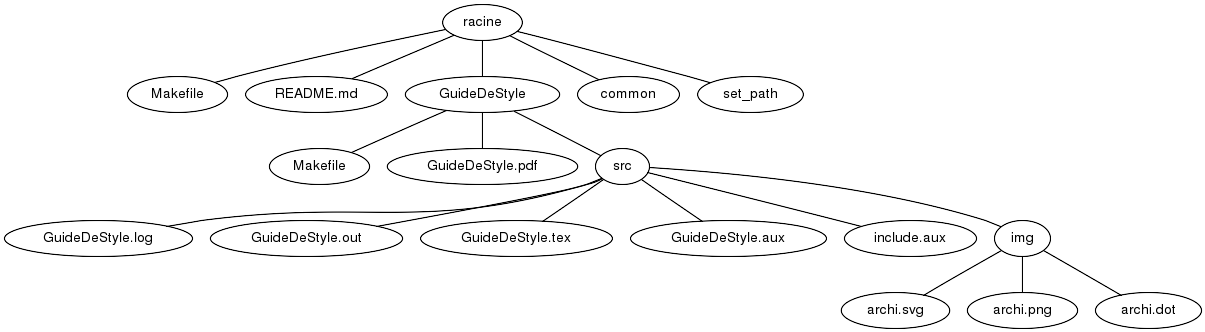
\includegraphics[width=\textwidth]{img/archi.png}
\caption{Organisation typique des dossiers, avec un livrable.}
\end{figure}
\end{document}
